\documentclass[12pt,]{tufte-book}

% ams
\usepackage{amssymb,amsmath}

\usepackage{ifxetex,ifluatex}
\usepackage{fixltx2e} % provides \textsubscript
\ifnum 0\ifxetex 1\fi\ifluatex 1\fi=0 % if pdftex
  \usepackage[T1]{fontenc}
  \usepackage[utf8]{inputenc}
\else % if luatex or xelatex
  \makeatletter
  \@ifpackageloaded{fontspec}{}{\usepackage{fontspec}}
  \makeatother
  \defaultfontfeatures{Ligatures=TeX,Scale=MatchLowercase}
  \makeatletter
  \@ifpackageloaded{soul}{
     \renewcommand\allcapsspacing[1]{{\addfontfeature{LetterSpace=15}#1}}
     \renewcommand\smallcapsspacing[1]{{\addfontfeature{LetterSpace=10}#1}}
   }{}
  \makeatother

\fi

% graphix
\usepackage{graphicx}
\setkeys{Gin}{width=\linewidth,totalheight=\textheight,keepaspectratio}

% booktabs
\usepackage{booktabs}

% url
\usepackage{url}

% hyperref
\usepackage{hyperref}

% units.
\usepackage{units}


\setcounter{secnumdepth}{2}

% citations


% pandoc syntax highlighting
\usepackage{color}
\usepackage{fancyvrb}
\newcommand{\VerbBar}{|}
\newcommand{\VERB}{\Verb[commandchars=\\\{\}]}
\DefineVerbatimEnvironment{Highlighting}{Verbatim}{commandchars=\\\{\}}
% Add ',fontsize=\small' for more characters per line
\newenvironment{Shaded}{}{}
\newcommand{\AlertTok}[1]{\textcolor[rgb]{1.00,0.00,0.00}{\textbf{#1}}}
\newcommand{\AnnotationTok}[1]{\textcolor[rgb]{0.38,0.63,0.69}{\textbf{\textit{#1}}}}
\newcommand{\AttributeTok}[1]{\textcolor[rgb]{0.49,0.56,0.16}{#1}}
\newcommand{\BaseNTok}[1]{\textcolor[rgb]{0.25,0.63,0.44}{#1}}
\newcommand{\BuiltInTok}[1]{\textcolor[rgb]{0.00,0.50,0.00}{#1}}
\newcommand{\CharTok}[1]{\textcolor[rgb]{0.25,0.44,0.63}{#1}}
\newcommand{\CommentTok}[1]{\textcolor[rgb]{0.38,0.63,0.69}{\textit{#1}}}
\newcommand{\CommentVarTok}[1]{\textcolor[rgb]{0.38,0.63,0.69}{\textbf{\textit{#1}}}}
\newcommand{\ConstantTok}[1]{\textcolor[rgb]{0.53,0.00,0.00}{#1}}
\newcommand{\ControlFlowTok}[1]{\textcolor[rgb]{0.00,0.44,0.13}{\textbf{#1}}}
\newcommand{\DataTypeTok}[1]{\textcolor[rgb]{0.56,0.13,0.00}{#1}}
\newcommand{\DecValTok}[1]{\textcolor[rgb]{0.25,0.63,0.44}{#1}}
\newcommand{\DocumentationTok}[1]{\textcolor[rgb]{0.73,0.13,0.13}{\textit{#1}}}
\newcommand{\ErrorTok}[1]{\textcolor[rgb]{1.00,0.00,0.00}{\textbf{#1}}}
\newcommand{\ExtensionTok}[1]{#1}
\newcommand{\FloatTok}[1]{\textcolor[rgb]{0.25,0.63,0.44}{#1}}
\newcommand{\FunctionTok}[1]{\textcolor[rgb]{0.02,0.16,0.49}{#1}}
\newcommand{\ImportTok}[1]{\textcolor[rgb]{0.00,0.50,0.00}{\textbf{#1}}}
\newcommand{\InformationTok}[1]{\textcolor[rgb]{0.38,0.63,0.69}{\textbf{\textit{#1}}}}
\newcommand{\KeywordTok}[1]{\textcolor[rgb]{0.00,0.44,0.13}{\textbf{#1}}}
\newcommand{\NormalTok}[1]{#1}
\newcommand{\OperatorTok}[1]{\textcolor[rgb]{0.40,0.40,0.40}{#1}}
\newcommand{\OtherTok}[1]{\textcolor[rgb]{0.00,0.44,0.13}{#1}}
\newcommand{\PreprocessorTok}[1]{\textcolor[rgb]{0.74,0.48,0.00}{#1}}
\newcommand{\RegionMarkerTok}[1]{#1}
\newcommand{\SpecialCharTok}[1]{\textcolor[rgb]{0.25,0.44,0.63}{#1}}
\newcommand{\SpecialStringTok}[1]{\textcolor[rgb]{0.73,0.40,0.53}{#1}}
\newcommand{\StringTok}[1]{\textcolor[rgb]{0.25,0.44,0.63}{#1}}
\newcommand{\VariableTok}[1]{\textcolor[rgb]{0.10,0.09,0.49}{#1}}
\newcommand{\VerbatimStringTok}[1]{\textcolor[rgb]{0.25,0.44,0.63}{#1}}
\newcommand{\WarningTok}[1]{\textcolor[rgb]{0.38,0.63,0.69}{\textbf{\textit{#1}}}}

% table with pandoc
\usepackage{longtable,booktabs,array}
\usepackage{calc} % for calculating minipage widths
% Correct order of tables after \paragraph or \subparagraph
\usepackage{etoolbox}
\makeatletter
\patchcmd\longtable{\par}{\if@noskipsec\mbox{}\fi\par}{}{}
\makeatother
% Allow footnotes in longtable head/foot
\IfFileExists{footnotehyper.sty}{\usepackage{footnotehyper}}{\usepackage{footnote}}
\makesavenoteenv{longtable}

% multiplecol
\usepackage{multicol}

% strikeout
\usepackage[normalem]{ulem}

% morefloats
\usepackage{morefloats}


% tightlist macro required by pandoc >= 1.14
\providecommand{\tightlist}{%
  \setlength{\itemsep}{0pt}\setlength{\parskip}{0pt}}

% title / author / date
\title{Monte-Carlo\\
Methods}
\author{P. Henaff}
\date{2023-03-09}

% Preamble from Rmetrics

\usepackage{booktabs}
\usepackage{amsthm}
\usepackage{xfrac}
\makeatletter
\def\thm@space@setup{%
  \thm@preskip=8pt plus 2pt minus 4pt
  \thm@postskip=\thm@preskip
}
\makeatother

% Index
\usepackage{makeidx}
\makeindex

% binomial trees
\usepackage{pgfplots}
\usepackage{tikz}
\usetikzlibrary{shapes.multipart}
\usepackage{pgfplots}
\usetikzlibrary{shapes}
\usetikzlibrary{external}
\usepgfplotslibrary{external}
\usetikzlibrary{positioning}
\pgfplotsset{compat=1.18}

% R and other languages

\newcommand{\RR}{\textsf{R}}
\newcommand{\Rmetrics}{Rmetrics}

%\newcommand{`r to_index("", "functions")`}[1]{\texttt{#1()}\index{R~functions@\RR~functions!#1}}
%\newcommand{`r to_index("", "classes")`}[1]{\texttt{#1}}
%\newcommand{`r to_index("", "classes")`}[1]{\texttt{#1}\index{R~classes@\RR~classes!#1}}
%\newcommand{\pkg}[1]{\texttt{#1}\index{R~packages@\RR~packages!#1}}
%\newcommand{\dataset}[1]{\texttt{#1}\index{R~data@\RR~data!#1}}
%\newcommand{\code}[1]{\texttt{#1}\index{#1}}

% Preamble from VIP

\newcommand{\given}{\mid}
\renewcommand{\neg}{\mathbin{\sim}}
\renewcommand{\wedge}{\mathbin{\&}}
\renewcommand{\u}{U}
\newcommand{\gt}{>}
\newcommand{\p}{Pr}
\newcommand{\E}{E}
\newcommand{\EU}{EU}
\newcommand{\pr}{Pr}
\newcommand{\po}{Pr^*}
\newcommand{\degr}{^{\circ}}
\definecolor{bookred}{RGB}{228,6,19}
\definecolor{bookblue}{RGB}{0,92,169}
\definecolor{bookpurple}{RGB}{114,49,94}

\newenvironment{epigraph}%
{
\begin{flushright}
\begin{minipage}{20em}
\begin{flushright}
\itshape
}%
{
\end{flushright}
\end{minipage}
\end{flushright}
}
\newenvironment{problem}{\begin{quote}\normalsize}{\end{quote}}
\newenvironment{puzzle}{\begin{quote}\normalsize}{\end{quote}}
\def\argument{\list{}{\leftmargin3em}\item[]}
\let\endargument=\endlist
\usepackage{fontawesome}
\newenvironment{warning}{\begin{itemize}\item[\faBan]}{\end{itemize}}
\usepackage{marvosym}
\newenvironment{info}{\begin{itemize}\item[\Info]}{\end{itemize}}

%%%% Kevin Godny's code for title page and contents from https://groups.google.com/forum/#!topic/tufte-latex/ujdzrktC1BQ
\makeatletter
\renewcommand{\maketitlepage}{%
\begingroup%
\setlength{\parindent}{0pt}
{\fontsize{18}{18}\selectfont\textit{\@author}\par}
\vspace{1.75in}{\fontsize{36}{14}\selectfont\@title\par}
\vspace{0.5in}{\fontsize{20}{14}\selectfont with R and Rmetrics\par}
\vspace{0.5in}{\fontsize{14}{14}\selectfont\textsf{\smallcaps{v 2.0}}\par}
\vfill{\fontsize{14}{14}\selectfont\textit{An Open Access Publication}\par}
\thispagestyle{empty}
\endgroup
}
\makeatother

% Change shape from [display] to [block] to keep chapter numbers and titles on the same line
\titleformat{\chapter}%
  [block]% shape
  {\relax\ifthenelse{\NOT\boolean{@tufte@symmetric}}{\begin{fullwidth}}{}}% format applied to label+text
  {\itshape\huge\thechapter}% label
  {3em}% horizontal separation between label and title body
  {\huge\rmfamily\itshape}% before the title body
  [\ifthenelse{\NOT\boolean{@tufte@symmetric}}{\end{fullwidth}}{}]% after the title body


\usepackage{etoolbox}
% Jesse Rosenthal's code from https://groups.google.com/forum/#!topic/pandoc-discuss/wCF78X6SvwY
% Avoid new pagraph/indent after lists, quotes, etc.
\makeatletter
\newcommand{\gobblepars}{%
    \@ifnextchar\par%
        {\expandafter\gobblepars\@gobble}%
        {}}
\newcommand{\eatpar}{\@ifnextchar\par{\@gobble}{}}
\newcommand{\forcepar}{\par}
\makeatother
\AfterEndEnvironment{quote}{\expandafter\gobblepars}
\AfterEndEnvironment{enumerate}{\expandafter\gobblepars}
\AfterEndEnvironment{itemize}{\expandafter\gobblepars}
\AfterEndEnvironment{description}{\expandafter\gobblepars}
\AfterEndEnvironment{example}{\expandafter\gobblepars}
\AfterEndEnvironment{argument}{\expandafter\gobblepars}
\AfterEndEnvironment{problem}{\expandafter\gobblepars}
\AfterEndEnvironment{info}{\expandafter\gobblepars}
\AfterEndEnvironment{warning}{\expandafter\gobblepars}
\AfterEndEnvironment{marginfigure}{\expandafter\gobblepars}
\AfterEndEnvironment{longtable}{\expandafter\gobblepars} % not working, why?
\makeatletter
\AfterEndEnvironment{longtable}{\par\@afterindentfalse\@afterheading} % this seems to work instead
\makeatother

\renewcommand*\descriptionlabel[1]{\hspace\labelsep\normalfont\em #1.}

% prevent extra space when \newthought follows \section
% see: https://tex.stackexchange.com/questions/291746/tufte-latex-newthought-after-section
\makeatletter
\def\tuftebreak{%
  \if@nobreak\else
    \par
    \ifdim\lastskip<\tufteskipamount
      \removelastskip \penalty -100
      \tufteskip
    \fi
  \fi
}
\makeatother

% indent lists a bit
\usepackage{enumitem}
\setlist[1]{leftmargin=24pt}

\def\labelitemii{$\circ$}
\usepackage{subfig}

\begin{document}

\maketitle



{
\setcounter{tocdepth}{0}
\tableofcontents
}

\hypertarget{monte-carlo-methods}{%
\chapter{Monte Carlo Methods}\label{monte-carlo-methods}}

There are many instances in computational finance where one needs to compute
the expected value of some function of a multivariate random variable. One can think about an option on a basket of stocks, or an option where the payoff is determined by observations performed at regular intervals in time, and so forth.

\newthought{Monte Carlo} methods, in contrast to lattice methods such as trees, become particularly attractive as the dimension of the domain increases. This can be illustrated by considering the problem of evaluating a volume \(V\) in \(R^d\), by evaluating a function \(f(X)\) at \(N\) points such that \(N = k^d\) for some integer \(k\).
Along each axis, the \(k\) points are evenly spaced. If a mid-point integration algorithm is used, then the error is of the order of \(1/k\), and \(1/k^2\) if a trapezoidal rule is used. Therefore, with \(N\) function evaluations, the error will be \(O(N^{-1/d})\) or \(O(N^{-2/d})\), depending upon the integration rule.

In contrast, consider performing the same calculation by evaluating \(g(X)\) at \(N\) random points such that \(g(X) = 1 if X \in V\) and \(0\) otherwise. The estimate \(S_N\) of the volume is

\[
S_N = C_d \frac{1}{N} \sum_{i=1}^N f(X_i)
\]
where \(C_d\) is the volume of the hypercube of dimension \(d\) containing the sphere. An an estimation of the variance of the estimate is

\[
V_n^2 = \frac{N-1}{N} \left[ \frac{1}{N} \sum_i g(X_i)^2 - \left(\frac{1}{N} \sum_i g(X_i)\right)^2 \right]
\]
which shows, by the central limit theorem, that the error is a function of \(\sqrt{1/N}\), and not of the dimension of the domain.

\[
S_n - E(g(X)) \approx N(0, \sqrt{1/N} V_n)
\]

The following experiments contrast the lattice and Monte-Carlo methods. We estimate the volume of a sphere of radius 1 in \(R^d\) contained in an hypercube of the same dimension. The volume of the sphere is estimated by considering \(N\) points in \(R^d\) and determining if they are inside the sphere. Let \(K\) be the number of such points, the volume of the sphere is estimated as:

\[
V_N = \frac{K}{N} C_d
\]

The lattice and Monte-Carlo methods differ in the way the \(N\) points are chosen.
With the lattice algorithm, we construct a grid of \(N\) evenly spaced points in \(R^d\), while in the Monte-Carlo approach, those \(N\) points are drawn from a uniform multivariate distribution. Since we have an analytical expression for the volume of the sphere, we can readily observe the estimation error as a function of \(N\) and the dimension \(d\).

\begin{figure}
\subfloat[d=3\label{fig:dim-3-6-1}]{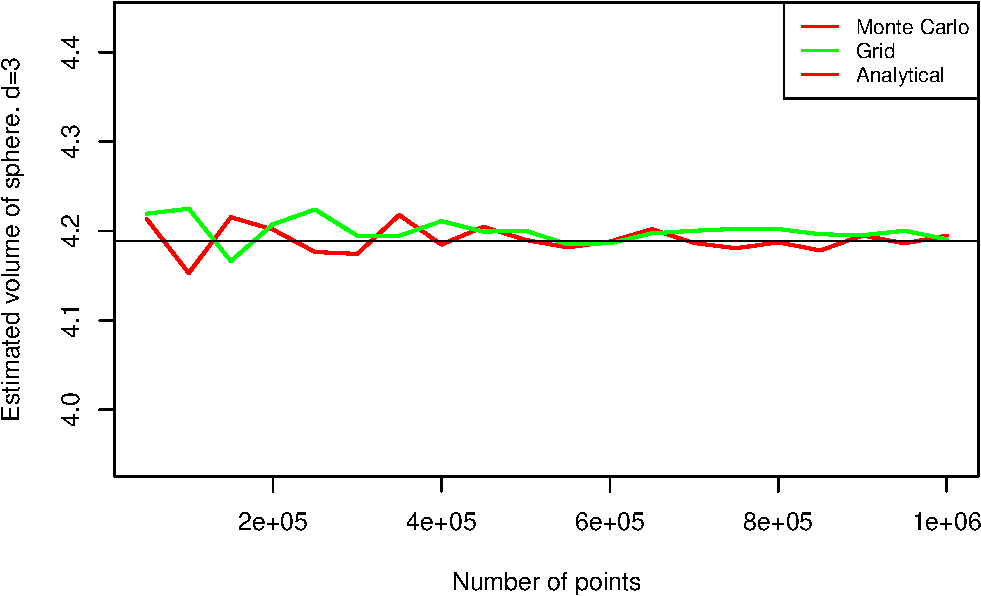
\includegraphics[width=0.45\linewidth]{800-MC-1_files/figure-latex/dim-3-6-1} }\subfloat[d=6\label{fig:dim-3-6-2}]{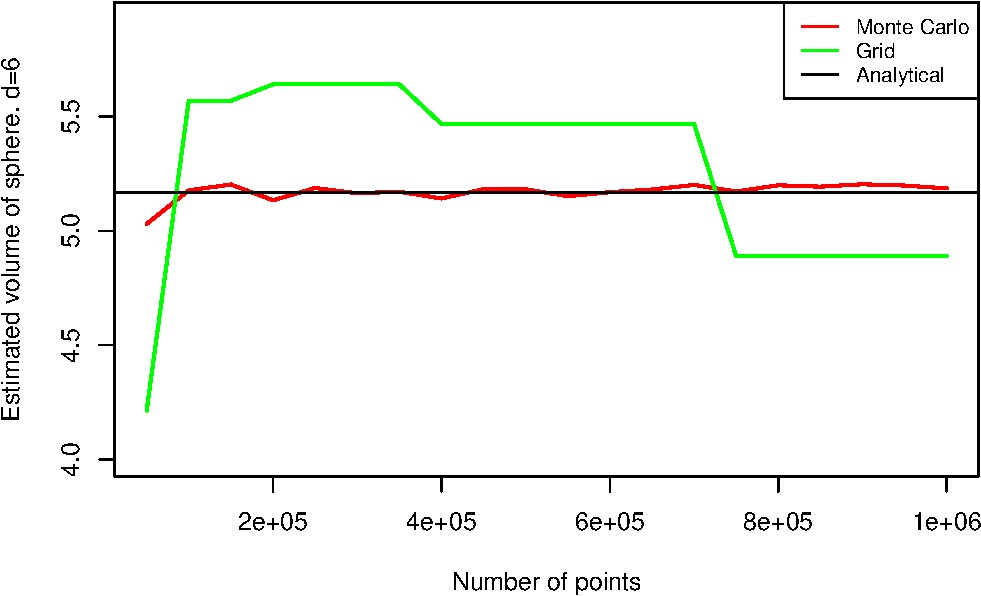
\includegraphics[width=0.45\linewidth]{800-MC-1_files/figure-latex/dim-3-6-2} }\caption[Calculation of the volume of a sphere in dimension 3 and 6, with an evenly spaced grid and Monte-Carlo simulation]{Calculation of the volume of a sphere in dimension 3 and 6, with an evenly spaced grid and Monte-Carlo simulation.}\label{fig:dim-3-6}
\end{figure}

For \(d=3\), the difference between the two methods is minimal.
In 6 dimensions, however, the superiority of the Monte Carlo algorithm becomes clearly visible. With \(10^6\) simulations, the Monte-Carlo error is \(O(1/\sqrt{N}) = 0.001\), but \(O(N^{-1/6}) = .1\) with the deterministic grid method. In 6 dimensions, with one million points, there are only 10 grid points per axis.

\newthought{Another reason} makes Monte-Carlo methods attractive in financial engineering, independently of the mathematical properties of the algorithm: a Monte-Carlo simulator, combined with a payoff language, forms a very flexible platform for pricing complex derivatives, without the need for ad-hoc software development. In addition, it provides the framework for easily testing the sensitivity of prices to asumptions regarding the underlying stochastic processes. All these resons make a Monte-Carlo pricing framework the tool of choice for structured products pricing and risk management.

\hypertarget{process-driven-sampling}{%
\section{Process-driven sampling}\label{process-driven-sampling}}

In computational finance, we typically need to simulate a stochastic process and evaluate a pricing function for each simulated path. In general terms, the stochastic differential equation to be discretized is

\[
dS_t = \mu(S_t, t)dt + \sigma(S_t, t)dW
\]
Integrating between \(t\) and \(t+\Delta t\) to get \(S_{t+\Delta t}\) gives:

\[
S_{t+\Delta t} = S_t + \int_t^{t+\Delta t} \mu(S_u, u) du + \int_T^{t+\Delta t} \sigma(S_u, u) dW_u
\label{eq:mc-1}
\]

Various schemes are available to discretize the integrals in \eqref{eq:mc-1}, Two popular schemes, the Euler and Milstein schemes, are next briefly compared.

\newthought{The Euler scheme} is the simplest way to approximate \eqref{eq:mc-1}: it amounts to approximate the integral using the left-point rule (since \(\mu(S_t, t)\) and \(\sigma(S_t, t)\) are known at time \(t\)). Nothing that

\begin{align}
\int_t^{t+\Delta t} \sigma(S-u, u) dW_u &\approx \sigma(S_t, t) \int dW_u \\
&\approx \sigma(S_t, t) \left(W_{t+\Delta t} - W_t \right) \\
&\approx \sigma(S_t, t) \sqrt{\Delta t} Z
\end{align}

with \(Z \sim N(0, 1)\).

The Euler scheme is thus:

\[
S_{t+\Delta t} = S_t + \mu(S_t, t) \Delta t + \sigma(S_t, t) \sqrt{\Delta t} Z
\label{eq:mc-2}
\]
For the geometric brownian motion

\[
dS_t = r S_t dt + \sigma S_t dW
\label{eq:mc-gbm}
\]
applying \eqref{eq:mc-2} gives

\[
S_{t+\Delta t} = S_t + rS_t dt + \sigma S_t \sqrt{\Delta t} Z
\]

Using Ito's lemma with \(f(S_t) = \ln(S_t)\), we obtain

\[
d \ln(S_t) = (r-\frac{1}{2} \sigma^2) dt + \sigma dW
\label{eq:mc-3}
\]
and the corresponding Euler scheme is

\[
\ln(S_{t+\Delta t}) = \ln(S_t) + (r - \frac{1}{2} \sigma^2) dt + \sigma \sqrt{\Delta t} Z
\]
\newthought{Milstein's scheme} will be considered in the case where \(\mu\) and \(\sigma\) are only functions of \(S_t\).

\[
dS_t = \mu(S_t) dt + \sigma(S_t) dW
\]

The accuracy of the discretization is improved by expanding \(\mu(S_t)\) and \(\sigma(S_t)\) using Ito's lemma. The resulting discretization scheme is

\[
S_{t+\Delta t} = S_t + \mu_t dt + \sigma_t \sqrt{\Delta t} Z + \frac{1}{2} \sigma'_t \sigma_t \Delta t (Z^2 - 1)
\]

Applied to \eqref{eq:mc-gbm}, the Milstein scheme add a corrective term to the discretization:

\[
S_{t+\Delta t} = S_t + r S_t \Delta t + \sigma \sqrt{\Delta t} Z + \frac{1}{2} \sigma^2 S_t \Delta t (Z^2 - 1)
\]

However, applied to \eqref{eq:mc-3}, with \(\mu(S_t) = r - \frac{\sigma^2}{2}\) and \(\sigma(S_t) = \sigma\), the scheme becomes

\[
\ln(S_{t+\Delta t}) = \ln(S_t) + (r - \frac{1}{2} \sigma^2) dt + \sigma \sqrt{\Delta t} Z
\label{eq:mc-4}
\]

which is identical to the Euler scheme. It is therefore common practice to use the discretization of \(\ln(S_t)\) provided by \eqref{eq:mc-4}.

The accuracy of the scheme can be investigated by testing the non-arbitrage condition

\[
E(S_T) = S_0 e^{rT}
\]

\begin{figure}
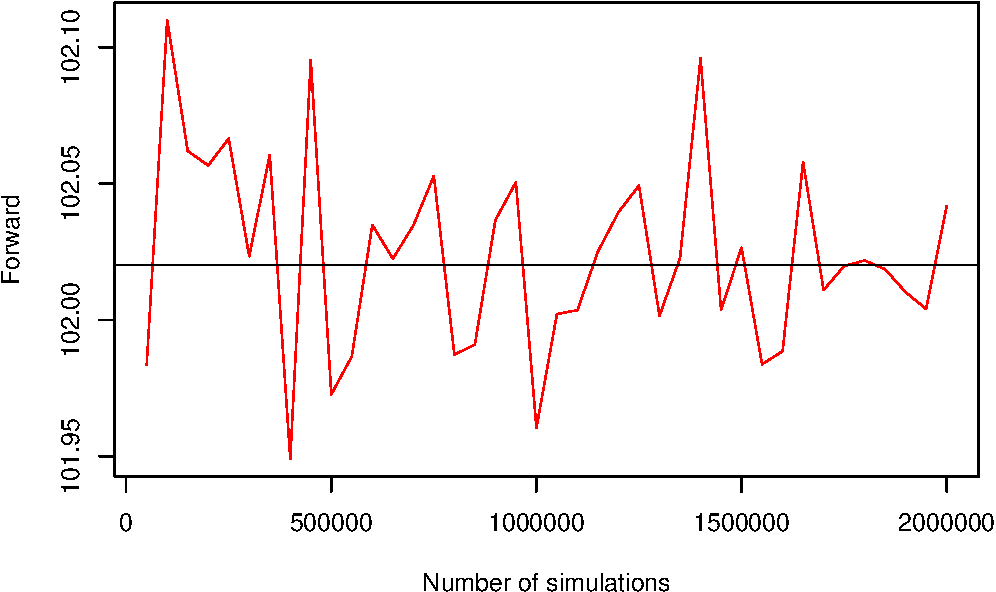
\includegraphics{800-MC-1_files/figure-latex/mc-forward-1} \caption[Expected value of ST as a function of the number of simulations]{Expected value of ST as a function of the number of simulations}\label{fig:mc-forward}
\end{figure}

Figure \ref{fig:mc-forward} shows the slow progress of \(E(S_T)\) towards the actual forward as the number of simulations increases. Clearly, a naive implementation of the discretization scheme is not satisfactory, and a variance reduction strategy is in order.

\hypertarget{variance-reduction}{%
\section{Variance Reduction}\label{variance-reduction}}

\newthought{Antithetic variates} is the simplest improvement to the discretization scheme. For an estimation with \(N\) trials, one draws \(N/2\) variates \(Z_i, i=1, \ldots, \frac{N}{2}\) from \(N(0,1)\), and sets \(Z_{N/2+i} = -Z_i, i=N/2+1, \ldots, N\). This has the double advantage of ensuring that \(E(Z)\) is exactly null, irrespective of \(N\), and also reduces the variance of the estimate. Consider the estimation of a parameter \(\theta = E(f(X))\) by Monte-Carlo simulation:

\[
\hat{\theta} = \frac{1}{N} \sum_i f(X_i)
\]
where the \(X_i\) are sampled according to the distribution of \(X\). With antithetic variates, the estimate is given by:

\begin{align}
\hat{\theta_1} &= \frac{2}{N} \sum_{i=1}^{N/2} f(X_i) \\
\hat{\theta_2} &= \frac{2}{N} \sum_{i=1}^{N/2} f(-X_i) \\
\hat{\theta} &= \frac{\theta_1 + \theta_2}{2}
\end{align}

and the variance of \(\hat{\theta}\) is

\begin{align}
V(\hat(\theta)) &= \frac{1}{4} \left[ V(\hat{\theta_1}) + V(\hat{\theta_2}) + 2 Cov(\theta_1, \theta_2) \right] \\
&= \frac{\sigma^2}{N} + \frac{1}{2} Cov(\theta_1, \theta_2)
\end{align}
where \(\sigma^2\) is the variance of \(f(X)\). The scheme will be beneficial as long as \(Cov(\theta_1, \theta_2) < 0\).

We apply this technique to the pricing of an ATM European call, strike \(K=100\) and maturity \(T=1\), and compare the standard error of the price estimate, with and without antithetic trials. The results are sumarized in Figure \ref{fig:mc-call-anti}. The effectiveness of the technique is clearly visible.

\begin{figure}
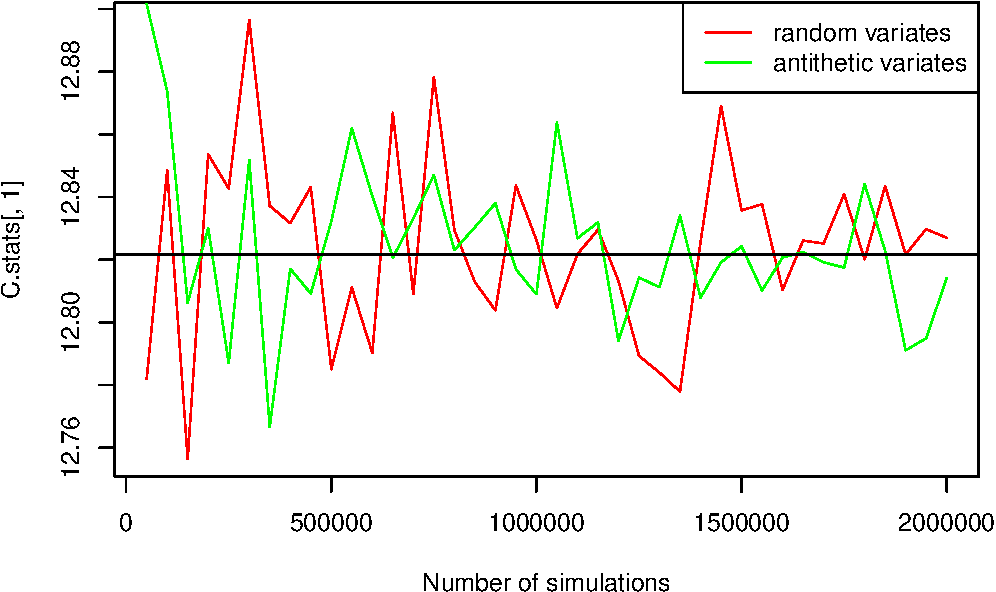
\includegraphics{800-MC-1_files/figure-latex/mc-call-anti-1} \caption[European call with and without antithetic variates]{European call with and without antithetic variates}\label{fig:mc-call-anti}
\end{figure}

\newthought{Quasi Random Sequences}

The discussion of algorithms for generating random or quasi-random numbers is outside the scope of these notes. It will be sufficient to remark that the use of quasi-random numbers such as Sobol sequences significantly improve the quality of the MC estimations.
A comparison of Sobol quasi-random numbers and the default uniform random sequence in two dimensions is shown in Figure @\ref(fig:rand). The Sobol variates are evenly distributed over the domain.

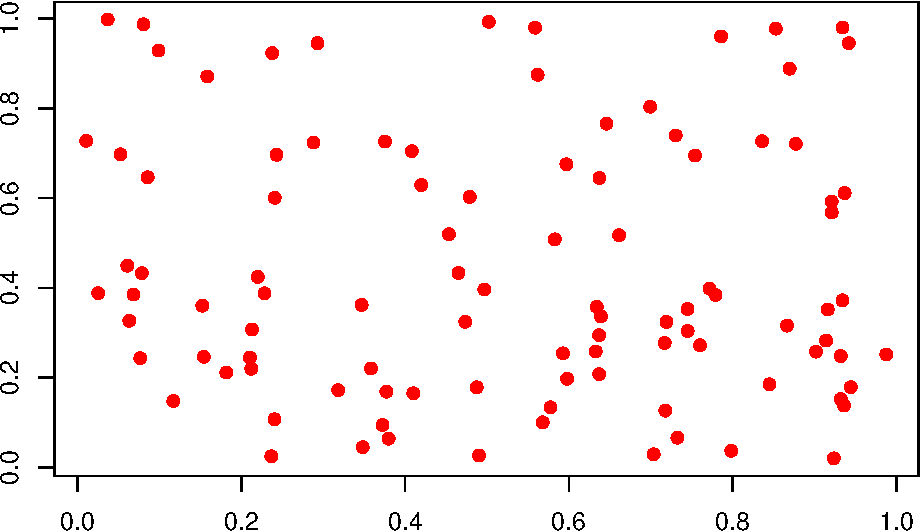
\includegraphics[width=0.45\linewidth]{800-MC-1_files/figure-latex/rand-1} 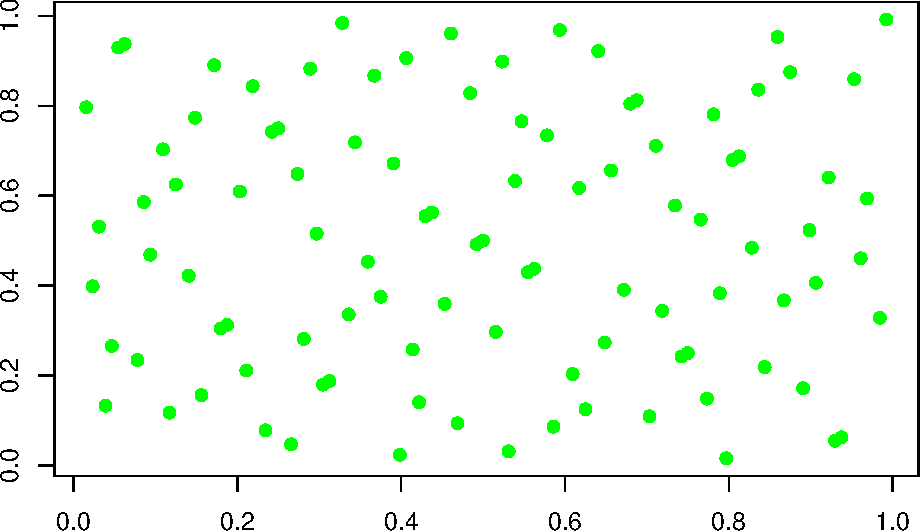
\includegraphics[width=0.45\linewidth]{800-MC-1_files/figure-latex/rand-2}

To appreciate the effect of a Sobol random number generator on the outcome of a MC simulation, we again estimate the forward price \(E(S_T)\), and compare the calculations performed with a Sobol sequence and with the other schemes considered so far. On these tests, the superiority of the antithetic scheme is apparent. Note that it does not make sense to construct antithetic variates from Sobol sequences, as this would disrupt the even distribution of the variates over the domain.

\begin{figure}
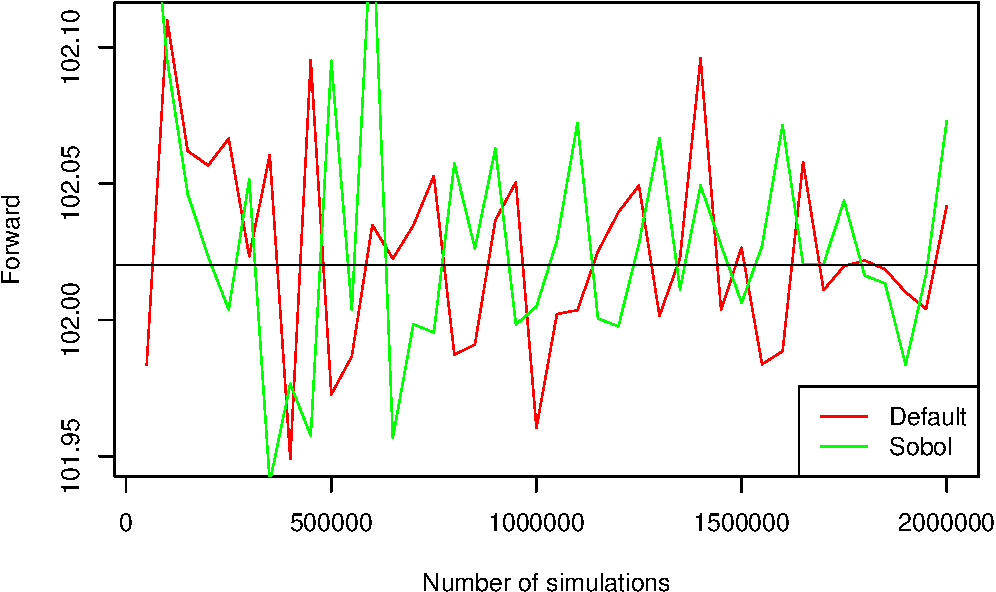
\includegraphics{800-MC-1_files/figure-latex/mc-forward-sobol-1} \caption[Expected value of ST as a function of the number of simulations]{Expected value of ST as a function of the number of simulations}\label{fig:mc-forward-sobol}
\end{figure}

\newthought{Importance Sampling}

The principe of importance sampling is to focus on the scenarios that comtribute to the average of the Monte-Carlo simulations, for instance, on the scenarios where an option expires in the money.

Pricing a financial asset amounts to computing

\[
P = \int_X p(X) \phi(X) dX
\]

where \(\phi(X)\) is the payoff, function of the state variables \(X\), and \(p(X)\) is the density of \(X\). Assume that \(\phi(X)\) only takes values in a subset \(A\) of the domain of \(X\), and let \(h(X)\) be the density of \(X\), restricted to the subset \(A\), we have:

\begin{align}
P &= \int_{X \in A} p(X) \phi(X) dX \\
&= \int_{X \in A} p(X) \frac{h(X)}{h(X)} \phi(X) dX \\
&= \int_{X \in A} h(X) \frac{p(X)}{h(X)} \phi(X) dX \\
&= E_h \left[ \frac{p(X)}{h(X)} \phi(X) \right]
\end{align}

Using \(N\) trials, with \(N_A\) scenarios in subset \(A\), the value \(P\) is estimated by:

\[
P \approx \frac{1}{N_A} \sum_{i=1}^{N_A} \frac{p(X_i)}{h(X_i)} \phi(X_i)
\]

Letś apply this algorithm to the pricing of an European call option with strike \(K\) and maturity \(T\) by Monte-Carlo simulation with \(N\) scenarios. The subset \(A\) consists of the \(N_A\) scenarios where \(S_T>K\). In this simple case, \(p(X)=1/N\), \(h(X)=1/N_A\) and the estimated call price, ignoring discounting, is

\[
P \approx \frac{1}{N} \sum_{i=1}^{N_A} (S_T^i - K)
\]
where \(S_T^i, i=1, \ldots, N_A\) are the scenarios ending in the money.

The standard error of this estimate is

\[
sd(P) =  \frac{\sqrt{N_A}}{N} sd(S_T)
\]

The effectiveness of this variance reduction technique is particularly clear when pricing out of the money options, as the following experiment illustrate.

\begin{Shaded}
\begin{Highlighting}[]
\NormalTok{K }\OtherTok{\textless{}{-}} \DecValTok{100}
\NormalTok{S}\FloatTok{.0} \OtherTok{\textless{}{-}} \DecValTok{102}
\NormalTok{T }\OtherTok{\textless{}{-}} \FloatTok{0.5}
\NormalTok{sigma }\OtherTok{\textless{}{-}}\NormalTok{ .}\DecValTok{2}
\NormalTok{r }\OtherTok{\textless{}{-}}\NormalTok{ .}\DecValTok{02}

\NormalTok{price.call }\OtherTok{\textless{}{-}} \ControlFlowTok{function}\NormalTok{(nb.sim) \{}
\NormalTok{Z }\OtherTok{\textless{}{-}} \FunctionTok{rnorm}\NormalTok{(nb.sim, }\AttributeTok{mean=}\DecValTok{0}\NormalTok{, }\AttributeTok{sd=}\DecValTok{1}\NormalTok{)}
\NormalTok{S.T }\OtherTok{=}\NormalTok{ S}\FloatTok{.0}\SpecialCharTok{*}\FunctionTok{exp}\NormalTok{((r }\SpecialCharTok{{-}} \FloatTok{0.5}\SpecialCharTok{*}\NormalTok{sigma}\SpecialCharTok{\^{}}\DecValTok{2}\NormalTok{)}\SpecialCharTok{*}\NormalTok{T }\SpecialCharTok{+} \FunctionTok{sqrt}\NormalTok{(T)}\SpecialCharTok{*}\NormalTok{sigma}\SpecialCharTok{*}\NormalTok{Z)}

\NormalTok{A.index }\OtherTok{\textless{}{-}}\NormalTok{ S.T }\SpecialCharTok{\textgreater{}}\NormalTok{ K}
\NormalTok{nb.A }\OtherTok{\textless{}{-}} \FunctionTok{sum}\NormalTok{(A.index)}
\NormalTok{call.payoff }\OtherTok{\textless{}{-}} \FunctionTok{pmax}\NormalTok{(S.T}\SpecialCharTok{{-}}\NormalTok{K, }\DecValTok{0}\NormalTok{)[A.index]}
\NormalTok{P.call.is }\OtherTok{\textless{}{-}} \FunctionTok{exp}\NormalTok{(}\SpecialCharTok{{-}}\NormalTok{r}\SpecialCharTok{*}\NormalTok{T) }\SpecialCharTok{*} \FunctionTok{mean}\NormalTok{(call.payoff) }\SpecialCharTok{*}\NormalTok{ nb.A }\SpecialCharTok{/}\NormalTok{ nb.sim}
\NormalTok{sd.call.is }\OtherTok{\textless{}{-}} \FunctionTok{exp}\NormalTok{(}\SpecialCharTok{{-}}\NormalTok{r}\SpecialCharTok{*}\NormalTok{T)}\SpecialCharTok{*} \FunctionTok{sqrt}\NormalTok{(nb.A) }\SpecialCharTok{*} \FunctionTok{sd}\NormalTok{(call.payoff) }\SpecialCharTok{/}\NormalTok{ nb.sim}

\NormalTok{call.payoff }\OtherTok{\textless{}{-}} \FunctionTok{pmax}\NormalTok{(S.T}\SpecialCharTok{{-}}\NormalTok{K, }\DecValTok{0}\NormalTok{)}
\NormalTok{P.call }\OtherTok{\textless{}{-}} \FunctionTok{exp}\NormalTok{(}\SpecialCharTok{{-}}\NormalTok{r}\SpecialCharTok{*}\NormalTok{T) }\SpecialCharTok{*} \FunctionTok{mean}\NormalTok{(call.payoff)}
\NormalTok{sd.call }\OtherTok{\textless{}{-}} \FunctionTok{sd}\NormalTok{(call.payoff)}\SpecialCharTok{/}\FunctionTok{sqrt}\NormalTok{(nb.sim)}
\FunctionTok{c}\NormalTok{(P.call.is, sd.call.is, P.call, sd.call)}
\NormalTok{\}}

\NormalTok{increment }\OtherTok{\textless{}{-}} \DecValTok{50000}
\NormalTok{nb.calcs }\OtherTok{\textless{}{-}} \DecValTok{20}
\NormalTok{sim.range }\OtherTok{\textless{}{-}}\NormalTok{ increment}\SpecialCharTok{*}\FunctionTok{seq}\NormalTok{(nb.calcs)}
\NormalTok{P.call }\OtherTok{\textless{}{-}} \FunctionTok{foreach}\NormalTok{(}\AttributeTok{i=}\DecValTok{1}\SpecialCharTok{:}\NormalTok{nb.calcs, }\AttributeTok{.combine=}\NormalTok{rbind) }\SpecialCharTok{\%dopar\%}\NormalTok{ \{}
\NormalTok{nb.sim }\OtherTok{\textless{}{-}}\NormalTok{ i}\SpecialCharTok{*}\NormalTok{increment}
\FunctionTok{price.call}\NormalTok{(nb.sim)}
\NormalTok{\}}
\NormalTok{P.BS }\OtherTok{\textless{}{-}} \FunctionTok{GBSOption}\NormalTok{(}\AttributeTok{TypeFlag=}\StringTok{"c"}\NormalTok{, }\AttributeTok{S=}\NormalTok{S}\FloatTok{.0}\NormalTok{, }\AttributeTok{X=}\NormalTok{K, }\AttributeTok{Time=}\NormalTok{T, }\AttributeTok{r=}\NormalTok{r, }\AttributeTok{b=}\NormalTok{r, }\AttributeTok{sigma=}\NormalTok{sigma)}\SpecialCharTok{@}\NormalTok{price}
\end{Highlighting}
\end{Shaded}

\begin{figure}
\subfloat[Importance Sampling\label{fig:unnamed-chunk-4-1}]{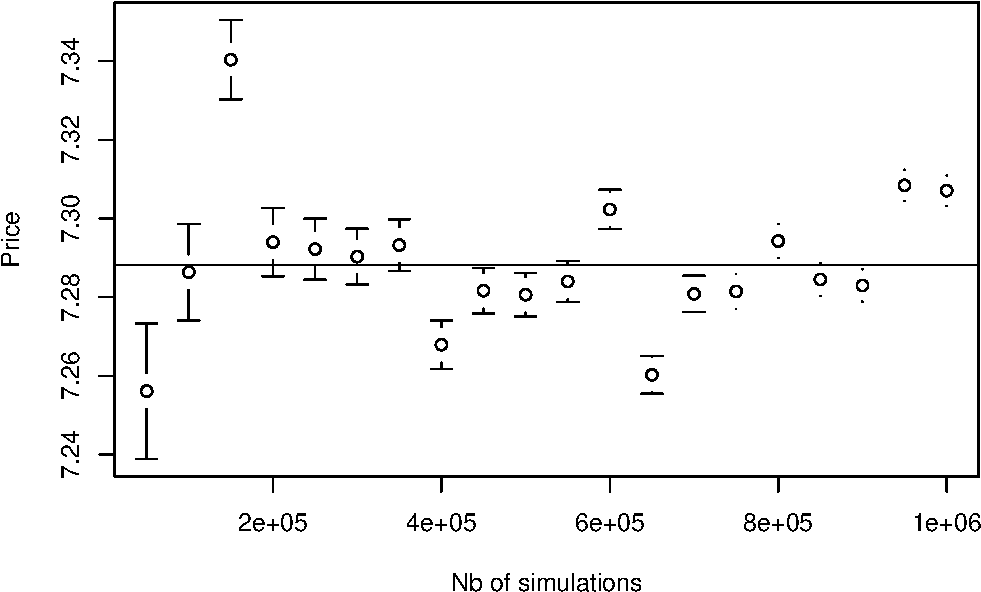
\includegraphics[width=0.45\linewidth]{800-MC-1_files/figure-latex/unnamed-chunk-4-1} }\subfloat[Simple MC\label{fig:unnamed-chunk-4-2}]{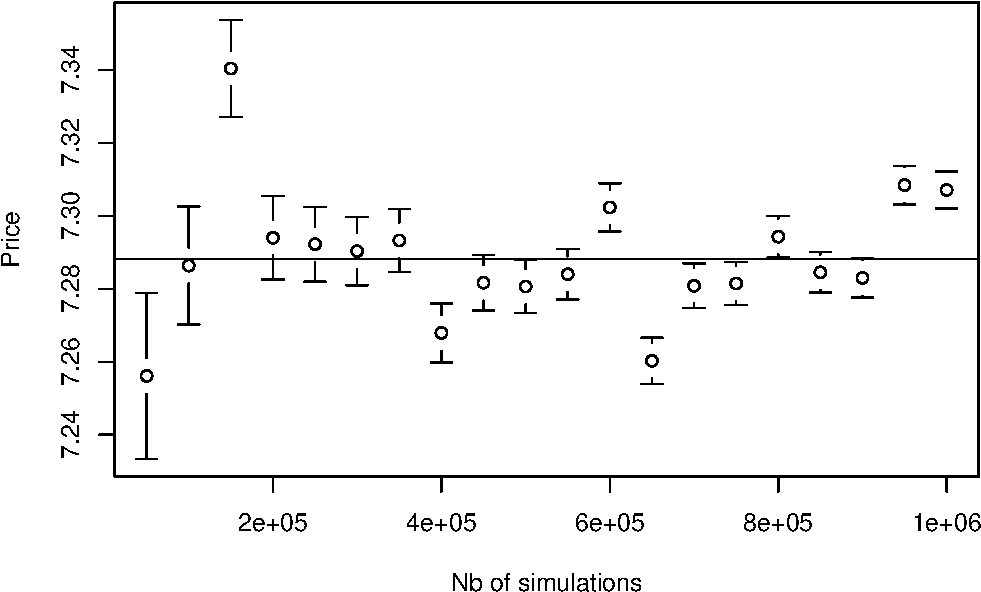
\includegraphics[width=0.45\linewidth]{800-MC-1_files/figure-latex/unnamed-chunk-4-2} }\caption[Pricing an European Option]{Pricing an European Option}\label{fig:unnamed-chunk-4}
\end{figure}

\newthought{Control Variates}

In many instances, we use MC simulations to price a complex product, and we are aware of simpler, related products for which there is an analytical solution.
That information can be useful to reduce the variance of our Monte-Carlo simulation.

Let \(g(X)\) be the payoff of the complex instrument to be priced by MC simulation:

\[
P_g = \frac{1}{N} \sum_i^n g(X_i)
\]
Let \(f(X)\) be the payoff of another instrument for which the expected value \(f^* = E(f)\) is known exactly. We can write:

\[
E \left[ \frac{1}{N} \sum_i g(X_i) \right] = E \left[ \frac{1}{N} \sum_i g(X_i) + \beta \left( f^* - \frac{1}{N} \sum_i f(X_i) \right) \right]
\]
and the estimator of \(P_g\) with the control variate correction is

\[
\hat{P_g} = \frac{1}{N} \sum_i \left[ g(X_i) + \beta (f^* - f(X_i)) \right]
\]
with the optimal \(\beta\) being

\[
\beta^* = \frac{Cov(f,g)}{V(g)}
\]

We illustrate the concept by pricing an Asian option (arithmetic average) and using a European option as control variate.

We create 5000 scenarios, with 50 observations per year.

\begin{Shaded}
\begin{Highlighting}[]
\NormalTok{dtExpiry }\OtherTok{\textless{}{-}} \FunctionTok{myDate}\NormalTok{(}\StringTok{\textquotesingle{}01jan2011\textquotesingle{}}\NormalTok{)}
\NormalTok{dtStart }\OtherTok{\textless{}{-}} \FunctionTok{myDate}\NormalTok{(}\StringTok{\textquotesingle{}01jan2010\textquotesingle{}}\NormalTok{)}
\NormalTok{nbSteps }\OtherTok{\textless{}{-}} \DecValTok{50}
\NormalTok{nbPaths }\OtherTok{\textless{}{-}} \DecValTok{100000}

\NormalTok{S}\FloatTok{.0} \OtherTok{\textless{}{-}} \DecValTok{100}
\NormalTok{sigma}\OtherTok{=}\NormalTok{.}\DecValTok{3}
\NormalTok{r}\OtherTok{=}\NormalTok{.}\DecValTok{01}
\NormalTok{T }\OtherTok{=} \FunctionTok{as.numeric}\NormalTok{(dtExpiry}\SpecialCharTok{{-}}\NormalTok{dtStart)}\SpecialCharTok{/}\DecValTok{365}

\NormalTok{dtSim }\OtherTok{\textless{}{-}} \FunctionTok{seq}\NormalTok{(}\FunctionTok{as.timeDate}\NormalTok{(dtStart), }\FunctionTok{as.timeDate}\NormalTok{(dtExpiry),}
             \AttributeTok{length.out=}\NormalTok{nbSteps}\SpecialCharTok{+}\DecValTok{1}\NormalTok{)}

\NormalTok{tSpot }\OtherTok{\textless{}{-}} \FunctionTok{pathSimulator}\NormalTok{(}\AttributeTok{dtSim =}\NormalTok{ dtSim, }\AttributeTok{nbPaths=}\NormalTok{nbPaths, }
    \AttributeTok{innovations.gen=}\NormalTok{sobolInnovations, }\AttributeTok{path.gen=}\NormalTok{logNormal, }
    \AttributeTok{path.param =} \FunctionTok{list}\NormalTok{(}\AttributeTok{mu=}\NormalTok{r, }\AttributeTok{sigma=}\NormalTok{sigma), }\AttributeTok{S0=}\NormalTok{S}\FloatTok{.0}\NormalTok{, }
    \AttributeTok{antithetic =}\NormalTok{ T, }
    \AttributeTok{standardization =}\NormalTok{ T, }\AttributeTok{trace =}\NormalTok{ F)}
\end{Highlighting}
\end{Shaded}

Next, we price an European call, strike 100, and compare the estimated price to the analytical value.

\begin{Shaded}
\begin{Highlighting}[]
\NormalTok{K }\OtherTok{\textless{}{-}} \DecValTok{100}
\NormalTok{EuroCall }\OtherTok{\textless{}{-}} \ControlFlowTok{function}\NormalTok{(x) \{}
  \FunctionTok{max}\NormalTok{(x[}\FunctionTok{length}\NormalTok{(x)]}\SpecialCharTok{{-}}\NormalTok{K,}\DecValTok{0}\NormalTok{)}
\NormalTok{\}}

\NormalTok{payoff.euro }\OtherTok{\textless{}{-}} \FunctionTok{apply}\NormalTok{(tSpot,}\DecValTok{2}\NormalTok{, }\AttributeTok{FUN=}\NormalTok{EuroCall)}\SpecialCharTok{*}\FunctionTok{exp}\NormalTok{(}\SpecialCharTok{{-}}\NormalTok{r}\SpecialCharTok{*}\NormalTok{T)}
\NormalTok{E.euro }\OtherTok{\textless{}{-}} \FunctionTok{mean}\NormalTok{(payoff.euro)}
\NormalTok{V.euro }\OtherTok{\textless{}{-}} \FunctionTok{var}\NormalTok{(payoff.euro)}

\NormalTok{A.euro }\OtherTok{\textless{}{-}} \FunctionTok{GBSOption}\NormalTok{(}\AttributeTok{TypeFlag =} \StringTok{"c"}\NormalTok{, S}\FloatTok{.0}\NormalTok{, }\AttributeTok{X =}\NormalTok{ K, }\AttributeTok{Time =}\NormalTok{ T, }\AttributeTok{r =}\NormalTok{ r, }
          \AttributeTok{b =}\NormalTok{ r, }\AttributeTok{sigma =}\NormalTok{ sigma)}\SpecialCharTok{@}\NormalTok{price}

\FunctionTok{print}\NormalTok{(}\FunctionTok{paste}\NormalTok{(}\StringTok{\textquotesingle{}European Call MC:\textquotesingle{}}\NormalTok{, }\FunctionTok{round}\NormalTok{(E.euro,}\DecValTok{3}\NormalTok{), }\StringTok{\textquotesingle{}+/{-}\textquotesingle{}}\NormalTok{,}
            \FunctionTok{round}\NormalTok{(}\FunctionTok{sqrt}\NormalTok{(V.euro}\SpecialCharTok{/}\NormalTok{nbPaths),}\DecValTok{3}\NormalTok{), }
            \StringTok{\textquotesingle{}BS:\textquotesingle{}}\NormalTok{, }\FunctionTok{round}\NormalTok{(A.euro,}\DecValTok{3}\NormalTok{)))}
\end{Highlighting}
\end{Shaded}

\begin{verbatim}
## [1] "European Call MC: 12.391 +/- 0.068 BS: 12.368"
\end{verbatim}

We next price a geometric Asian option and compare the estimate to an analytical expression

\begin{Shaded}
\begin{Highlighting}[]
\NormalTok{GeomAsianCall }\OtherTok{\textless{}{-}} \ControlFlowTok{function}\NormalTok{(x) \{}
\NormalTok{  avg }\OtherTok{\textless{}{-}} \FunctionTok{exp}\NormalTok{(}\FunctionTok{mean}\NormalTok{(}\FunctionTok{log}\NormalTok{(x)))}
  \FunctionTok{max}\NormalTok{(avg}\SpecialCharTok{{-}}\NormalTok{K, }\DecValTok{0}\NormalTok{)}
\NormalTok{\}}
\NormalTok{payoff.G.asian }\OtherTok{\textless{}{-}} \FunctionTok{apply}\NormalTok{(tSpot, }\DecValTok{2}\NormalTok{, }\AttributeTok{FUN=}\NormalTok{GeomAsianCall) }\SpecialCharTok{*} \FunctionTok{exp}\NormalTok{(}\SpecialCharTok{{-}}\NormalTok{r}\SpecialCharTok{*}\NormalTok{T)}
\NormalTok{E.G.asian }\OtherTok{\textless{}{-}} \FunctionTok{mean}\NormalTok{(payoff.G.asian)}
\NormalTok{V.G.asian }\OtherTok{\textless{}{-}} \FunctionTok{var}\NormalTok{(payoff.G.asian)}
\NormalTok{se.G.asian }\OtherTok{\textless{}{-}} \FunctionTok{sd}\NormalTok{(payoff.G.asian)}\SpecialCharTok{/}\FunctionTok{sqrt}\NormalTok{(nbPaths)}

\NormalTok{G.exact }\OtherTok{=} \FunctionTok{GeometricAverageRateOption}\NormalTok{(}\AttributeTok{TypeFlag=}\StringTok{"c"}\NormalTok{, }\AttributeTok{S=}\NormalTok{S}\FloatTok{.0}\NormalTok{, }\AttributeTok{X=}\NormalTok{K, }\AttributeTok{Time=}\NormalTok{T,}
                                     \AttributeTok{r=}\NormalTok{r, }\AttributeTok{b=}\NormalTok{r, }\AttributeTok{sigma=}\NormalTok{sigma)}\SpecialCharTok{@}\NormalTok{price}
\FunctionTok{print}\NormalTok{(}\FunctionTok{paste}\NormalTok{(}\StringTok{\textquotesingle{}European Geometric Asian Call MC:\textquotesingle{}}\NormalTok{, }\FunctionTok{round}\NormalTok{(E.G.asian,}\DecValTok{3}\NormalTok{),}
            \StringTok{\textquotesingle{}+/{-}\textquotesingle{}}\NormalTok{, }\FunctionTok{round}\NormalTok{(se.G.asian,}\DecValTok{3}\NormalTok{), }\StringTok{\textquotesingle{}Exact:\textquotesingle{}}\NormalTok{, }\FunctionTok{round}\NormalTok{(G.exact,}\DecValTok{3}\NormalTok{)))}
\end{Highlighting}
\end{Shaded}

\begin{verbatim}
## [1] "European Geometric Asian Call MC: 6.708 +/- 0.035 Exact: 6.701"
\end{verbatim}

We then price the Asian option by simulation.

\begin{Shaded}
\begin{Highlighting}[]
\NormalTok{EuroAsianCall }\OtherTok{\textless{}{-}} \ControlFlowTok{function}\NormalTok{(x) \{}
  \FunctionTok{max}\NormalTok{(}\FunctionTok{mean}\NormalTok{(x)}\SpecialCharTok{{-}}\NormalTok{K,}\DecValTok{0}\NormalTok{)}
\NormalTok{\}}

\NormalTok{payoff.asian }\OtherTok{\textless{}{-}} \FunctionTok{apply}\NormalTok{(tSpot, }\DecValTok{2}\NormalTok{, }\AttributeTok{FUN=}\NormalTok{EuroAsianCall) }\SpecialCharTok{*} \FunctionTok{exp}\NormalTok{(}\SpecialCharTok{{-}}\NormalTok{r}\SpecialCharTok{*}\NormalTok{T)}
\NormalTok{E.asian }\OtherTok{\textless{}{-}} \FunctionTok{mean}\NormalTok{(payoff.asian)}
\NormalTok{V.asian }\OtherTok{\textless{}{-}} \FunctionTok{var}\NormalTok{(payoff.asian)}
\NormalTok{se.asian }\OtherTok{\textless{}{-}} \FunctionTok{sd}\NormalTok{(payoff.asian)}\SpecialCharTok{/}\FunctionTok{sqrt}\NormalTok{(nbPaths)}

\FunctionTok{print}\NormalTok{(}\FunctionTok{paste}\NormalTok{(}\StringTok{\textquotesingle{}European Asian Call MC:\textquotesingle{}}\NormalTok{, }\FunctionTok{round}\NormalTok{(E.asian,}\DecValTok{3}\NormalTok{),}
            \StringTok{\textquotesingle{}+/{-}\textquotesingle{}}\NormalTok{, }\FunctionTok{round}\NormalTok{(se.asian,}\DecValTok{3}\NormalTok{)))}
\end{Highlighting}
\end{Shaded}

\begin{verbatim}
## [1] "European Asian Call MC: 7.117 +/- 0.037"
\end{verbatim}

Finally, we correct the Monte-Carlo estimate with the control variates, by first estimating the optimal \(\beta\) coefficient.

\begin{Shaded}
\begin{Highlighting}[]
\NormalTok{beta }\OtherTok{\textless{}{-}} \FunctionTok{cov}\NormalTok{(payoff.asian, payoff.G.asian) }\SpecialCharTok{/} \FunctionTok{var}\NormalTok{(payoff.G.asian)}
\NormalTok{payoff.asian.cv }\OtherTok{\textless{}{-}}\NormalTok{ payoff.asian }\SpecialCharTok{+}\NormalTok{ beta}\SpecialCharTok{*}\NormalTok{(G.exact}\SpecialCharTok{{-}}\NormalTok{payoff.G.asian) }

\NormalTok{E.asian.cv }\OtherTok{\textless{}{-}} \FunctionTok{mean}\NormalTok{(payoff.asian.cv)}
\NormalTok{se.asian.cv }\OtherTok{\textless{}{-}} \FunctionTok{stdev}\NormalTok{(payoff.asian.cv)}\SpecialCharTok{/}\FunctionTok{sqrt}\NormalTok{(nbPaths)}
\FunctionTok{print}\NormalTok{(}\FunctionTok{paste}\NormalTok{(}\StringTok{\textquotesingle{}Asian price with CV: \textquotesingle{}}\NormalTok{ , }\FunctionTok{round}\NormalTok{(E.asian.cv,}\DecValTok{3}\NormalTok{), }
            \StringTok{\textquotesingle{} SE: \textquotesingle{}}\NormalTok{, }\FunctionTok{round}\NormalTok{(se.asian.cv,}\DecValTok{3}\NormalTok{),}
            \StringTok{\textquotesingle{} beta: \textquotesingle{}}\NormalTok{, }\FunctionTok{round}\NormalTok{(beta,}\DecValTok{2}\NormalTok{)))}
\end{Highlighting}
\end{Shaded}

\begin{verbatim}
## [1] "Asian price with CV:  7.11  SE:  0.001  beta:  1.06"
\end{verbatim}


\printindex

\end{document}
